\documentclass{article}

\usepackage{graphicx}
\usepackage{color}
\usepackage{tikz}
\usepackage{pgfplots}
% \usepackage{pgf-umlsd}
\usepackage{ifthen}

\pgfplotsset{compat=1.7}
\pgfrealjobname{survey}
\begin{document}
\beginpgfgraphicnamed{flownet}
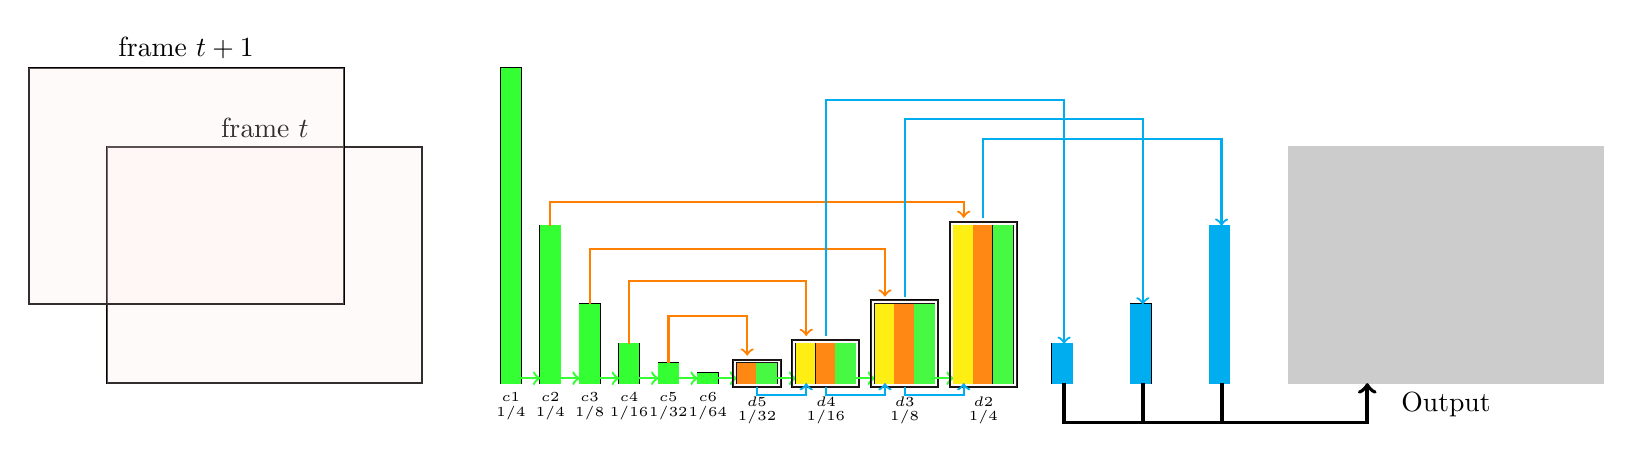
\begin{tikzpicture}[scale=1]
  % \draw[use as bounding box, transparent] (-1.8,-1.8) rectangle (17.2, 3.2);

  % Define the macro.
  % 1st argument: Height and width of the layer rectangle slice.
  % 2nd argument: Depth of the layer slice
  % 3rd argument: X Offset --> use it to offset layers from previously drawn layers.
  % 4th argument: Options for filldraw.
  % 5th argument: Text to be placed below this layer.
  % 6th argument: Y Offset --> Use it when an output needs to be fed to multiple layers that are on the same X offset.

  \newcommand{\networkLayer}[6]{
    \def\a{#1} % Used to distinguish input resolution for current layer.
    \def\b{#2}
    \def\c{#3} % Width of the cube to distinguish number of input channels for current layer.
    \def\d{#4} % X offset for current layer.
    % \ifthenelse {\equal{#6} {}} {\def\y{0}} {\def\y{#6}} % Y offset for current layer.

    % Draw the layer body.
    % back plane
    \draw[line width=0.25mm](\a,\b) rectangle (\a+\c,\b+\d) ;
    \draw (\a,\b) --node[midway,below] {#5}  (\a+\c,\b); 
    \ifthenelse {\equal{#6} {}}
    {} 
    {\filldraw[#6] (\a,\b) rectangle (\a+\c,\b+\d);}
  }

  \newcommand{\networkLayerA}[6]{
    \def\a{#1} % Used to distinguish input resolution for current layer.
    \def\b{#2}
    \def\c{#3} % Width of the cube to distinguish number of input channels for current layer.
    \def\d{#4} % X offset for current layer.
    % \ifthenelse {\equal{#6} {}} {\def\y{0}} {\def\y{#6}} % Y offset for current layer.

    % Draw the layer body.
    % back plane
    \draw[line width=0.25mm](\a,\b) rectangle (\a+\c,\b+\d) ;
    \draw (\a,\b+\d) --node[midway,above] {#5}  (\a+\c,\b+\d); 
    \ifthenelse {\equal{#6} {}}
    {} 
    {\filldraw[#6] (\a,\b) rectangle (\a+\c,\b+\d);}
  }

  % INPUT
  \networkLayerA{0.0}{0.0}{4}{3}{frame $t$}{opacity=0.2,color=red!10}
  \networkLayerA{-1.0}{1.0}{4}{3}{frame $t+1$}{opacity=0.2,color=red!10}
  
  % Encode
  \networkLayer{5.0}{0.0}{.25}{4}{\tiny{${c1} \atop 1/4$}}{color=green!80}
  \networkLayer{5.5}{0.0}{.25}{2}{\tiny{${c2} \atop 1/4$}}{color=green!80}
  \networkLayer{6.0}{0.0}{.25}{1}{\tiny{${c3} \atop 1/8$}}{color=green!80}
  \networkLayer{6.5}{0.0}{.25}{0.5}{\tiny{${c4} \atop 1/16$}}{color=green!80}
  \networkLayer{7.0}{0.0}{.25}{0.25}{\tiny{${c5} \atop 1/32$}}{color=green!80}
  \networkLayer{7.5}{0.0}{.25}{0.125}{\tiny{${c6} \atop 1/64$}}{color=green!80}
  \draw[->,line width=.3mm,green!80] (5.25,0.0625)--(5.5,0.0625);
  \draw[->,line width=.3mm,green!80] (5.75,0.0625)--(6.0,0.0625);
  \draw[->,line width=.3mm,green!80] (6.25,0.0625)--(6.5,0.0625);
  \draw[->,line width=.3mm,green!80] (6.75,0.0625)--(7.0,0.0625);
  \draw[->,line width=.3mm,green!80] (7.25,0.0625)--(7.5,0.0625);
  \draw[->,line width=.3mm,green!80] (7.50,0.0625)--(8.0,0.0625);

  % Decode
  \networkLayer{8.00}{0.0}{.25}{0.25}{}{color=orange}  
  \networkLayer{8.25}{0.0}{.25}{0.25}{}{color=green!80}
  \networkLayer{8.00-0.05}{-0.05}{.6}{0.35}{\tiny{$d5 \atop 1/32$}}{opacity=0.1,color=red!20}
  \draw[->,line width=.3mm,green!80] (8.5,0.0625)--(8.75,0.0625);
  \coordinate (a1) at (8.25,-0.05);   
  \coordinate (d5) at (8.125,0.35);   
                               
  \networkLayer{8.75}{0.0}{.25}{0.5}{}{color=yellow}
  \networkLayer{9.00}{0.0}{.25}{0.5}{}{color=orange}
  \networkLayer{9.25}{0.0}{.25}{0.5}{}{color=green!80}
  \networkLayer{8.75-0.05}{-0.05}{.85}{0.6}{\tiny{$d4 \atop 1/16$}}{opacity=0.1,color=red!20}
  \draw[->,line width=.3mm,green!80] (9.5,0.0625)--(9.75,0.0625);
  \coordinate (b2) at (8.875,0.0);   
  \coordinate (a2) at (9.125,-0.05);   
  \coordinate (d4) at (8.875,0.6);
   
  \networkLayer{9.75}{0.0}{.25}{1.0}{}{color=yellow}
  \networkLayer{10.0}{0.0}{.25}{1.0}{}{color=orange}
  \networkLayer{10.25}{0.0}{.25}{1.0}{}{color=green!80}
  \networkLayer{9.75-0.05}{-0.05}{.85}{1.1}{\tiny{$d3 \atop 1/8$}}{opacity=0.1,color=red!20}
  \draw[->,line width=.3mm,green!80] (10.5,0.0625)--(10.75,0.0625);
  \coordinate (b3) at (9.875,0.0);   
  \coordinate (a3) at (10.125,-0.05);   
  \coordinate (d3) at (9.875,1.1);   

  \networkLayer{10.75}{0.0}{.25}{2.0}{}{color=yellow}
  \networkLayer{11.00}{0.0}{.25}{2.0}{}{color=orange}
  \networkLayer{11.25}{0.0}{.25}{2.0}{}{color=green!80}
  \networkLayer{10.75-0.05}{-0.05}{.85}{2.1}{\tiny{$d2 \atop 1/4$}}{opacity=0.1,color=red!20}
  \coordinate (b4) at (10.875,0.0);   
  \coordinate (a4) at (11.125,-0.05);   
  \coordinate (d2) at (10.875,2.1);   
  
  \draw [->,thick,cyan] (a1) -- ++(-0.00,-0.1) -| (b2);               
  \draw [->,thick,cyan] (a2) -- ++(-0.00,-0.1) -| (b3);   
  \draw [->,thick,cyan] (a3) -- ++(-0.00,-0.1) -| (b4); 

  \coordinate (c2) at (5.625, 2.0);
  \coordinate (c3) at (6.125, 1.0);
  \coordinate (c4) at (6.625, 0.5);
  \coordinate (c5) at (7.125, 0.25);
  \draw [->,thick,orange] (c5) -- ++(-0.00,0.6) -| (d5); 
  \draw [->,thick,orange] (c4) -- ++(-0.00,0.8) -| (d4); 
  \draw [->,thick,orange] (c3) -- ++(-0.00,0.7) -| (d3); 
  \draw [->,thick,orange] (c2) -- ++(-0.00,0.3) -| (d2); 
  % Upsample
  \networkLayer{12.0}{0.0}{.25}{0.5}{}{color=cyan}
  \networkLayer{13.0}{0.0}{.25}{1.0}{}{color=cyan}
  \networkLayer{14.0}{0.0}{.25}{2.0}{}{color=cyan}
  \coordinate (u1) at (12.15,0.5);
  \coordinate (u2) at (13.15,1.0);
  \coordinate (u3) at (14.15,2.0);

  \coordinate (d4) at (9.125,0.6);
  \coordinate (d3) at (10.125,1.1);
  \coordinate (d2) at (11.125,2.1);
  \draw [->,thick,cyan] (d4) -- ++(0,3.0) -| (u1); 
  \draw [->,thick,cyan] (d3) -- ++(0,2.25) -| (u2); 
  \draw [->,thick,cyan] (d2) -- ++(0,1.0)  -| (u3);   
  
  % Output
  \networkLayer{15.0}{0.0}{4}{3}{Output}{color=black!20}
  \coordinate (u1) at (12.15,0.0);
  \coordinate (u2) at (13.15,0.0);
  \coordinate (u3) at (14.15,0.0);
  \coordinate (o1) at (16.00,0.0);
  \draw[->,line width=0.5mm] (u1) -- ++(0,-0.5) -| (o1);
  \draw[line width=0.5mm] (u2) -- ++(0,-0.5);
  \draw[line width=0.5mm] (u3) -- ++(0,-0.5);
\end{tikzpicture}
\endpgfgraphicnamed  
\end{document}
